
\documentclass[a4paper,12pt]{article} % добавить leqno в [] для нумерации слева

\usepackage[left=2cm,right=2cm,
top=2cm,bottom=2cm,bindingoffset=0cm]{geometry}

\usepackage{amsmath,amsfonts,amssymb,amsthm,mathtools} % AMS
\usepackage{icomma} 
\mathtoolsset{showonlyrefs=true} % Показывать номера только у тех формул, на которые есть \eqref{} в тексте.
\usepackage{euscript}	 % Шрифт Евклид
\usepackage{mathrsfs} % Красивый матшрифт
\usepackage{enumitem}
\usepackage{siunitx}
\usepackage{tikz} % To generate the plot from csv
\usepackage{pgfplots}
\usepackage{gensymb}

%%% Заголовок
\author{Kseniia Kasianova}
\title{Macroeconomics. Homework 1}
\date{\today}

\newcommand{\latinword}[1]{\textsf{\itshape #1}}

\setenumerate{label=\Alph*)}% global settings

\begin{document}

{\color{blue} \latinword{Begin to write your assignment here}}

\noindent\makebox[\linewidth]{\rule{\textwidth}{0.4pt}}


\section*{Test 2}
\subsection*{Problem 1}

Suppose, consumption function is represented by $ C = 200 + c(Y - T)$, $ I = 100 $ and government budget is balanced $G = T = 100 $


\begin{enumerate} 
	\item 
	The Keynesian equilibrium.

 \begin{enumerate} [label=\arabic*)] 
		
	\item 
	The expression of the planned expenditure as a function of income:

	$ PE = C + I + G = 200 + c\cdot (Y - 100) + 100 + 100 = 400 + c\cdot Y - c \cdot 100
 $

\item The relationship for c = 0.75. 


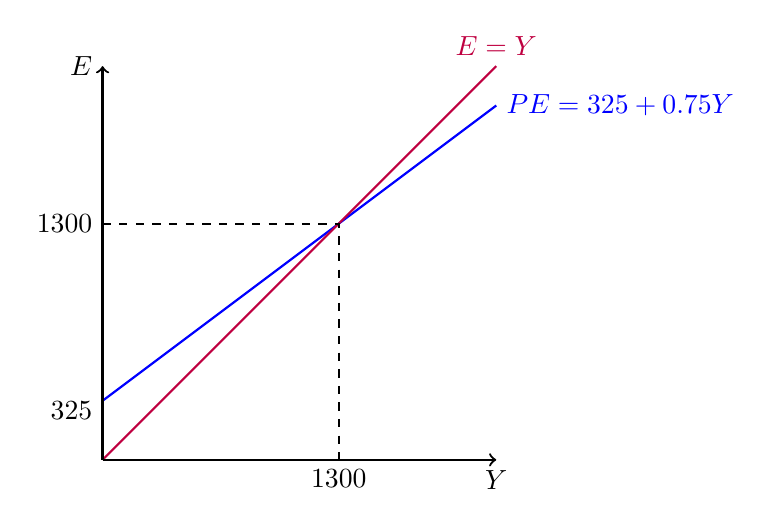
\begin{tikzpicture}[domain=0:5,scale=1,thick]
\usetikzlibrary{calc}   %allows coordinate calculations.

%Define linear parameters 
\def\dint{0.75}        %Y-intercept for DEMAND.
\def\dslp{0.75}         %Slope for DEMAND.
\def\sint{0}          %Y-intercept for SUPPLY.
\def\sslp{1}          %Slope for SUPPLY.
\def\demand{\x,{\dslp*\x+\dint}}
\def\supply{\x,{\sslp*\x+\sint}}

% Define coordinates
\coordinate (pfq) at  (3.75,0);
\coordinate (pfp) at  (3.75,3.625);
\coordinate (sfq) at  (0,3.625);

% DEMAND
\draw[thick,color=blue] plot (\demand) node[right] {$PE = 325 + 0.75Y $};

% SUPPLY
\draw[thick,color=purple] plot (\supply) node[above] {$ E = Y $};

% Draw axes, and dotted equilibrium lines.
\draw[->] (0,0) -- (5,0) node[below] {$Y$};
\draw[->] (0,0) -- (0,5) node[left] {$E$};

%Price floor and ceiling lines
\draw[dashed] (0,3) -- (3, 3) -- (3,0) node[below] {$1300$};
\node [left] at (0,0.625) {$ 325 $};
\node [left] at (0,3) {$ 1300 $};

\end{tikzpicture}


In the Keynesian cross diagram,  equilibrium occurs, where planned expenditure curve (shown in blue) intersects  a line that represents the equality of total income and output (shown in red). At this point total demand, PE, equals the total amount of national output, Y, so total demand equals total supply.

\item 
The intersection gives the equilibrium output, $ 1300 $.

\item 
Combining that we get: 
\begin{gather*}
E = C + I + G = 200 + 0.75 \cdot (Y - 100) + 100 + 100 = 325 + 0.75Y\\
Y = E \\
Y = 325 + 0.75Y\\
Y = 1300
\end{gather*}

\newpage

\item In Keynesian cross we have $ E = 400 + c\cdot Y - c \cdot T $.
An increase in MPC would shift the PE curve down, because of $- c \cdot T $ term, and make the curve steeper, because of $ c\cdot Y $ term. 


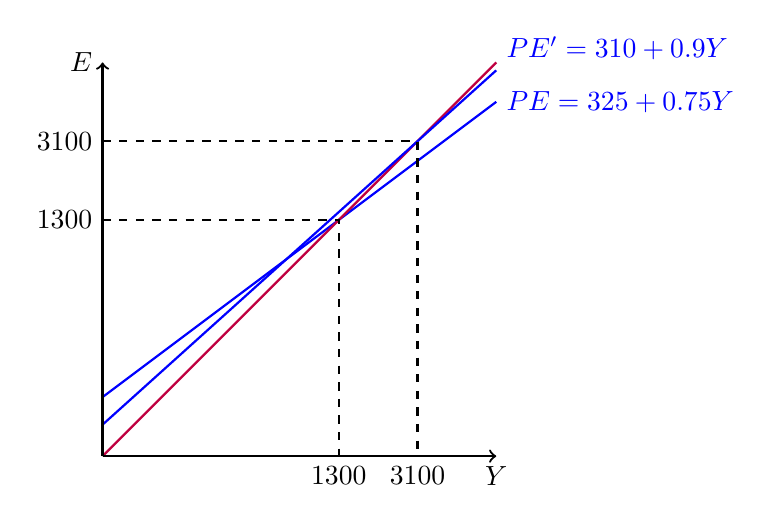
\begin{tikzpicture}[domain=0:5,scale=1,thick]
\usetikzlibrary{calc}   %allows coordinate calculations.

%Define linear parameters 
\def\dint{0.75}        %Y-intercept for DEMAND.
\def\dslp{0.75}         %Slope for DEMAND.
\def\sint{0}          %Y-intercept for SUPPLY.
\def\sslp{1}          %Slope for SUPPLY.
\def\demand{\x,{\dslp*\x+\dint}}
\def\supply{\x,{\sslp*\x+\sint}}

% Define coordinates
\coordinate (pfq) at  (3.75,0);
\coordinate (pfp) at  (3.75,3.625);
\coordinate (sfq) at  (0,3.625);

% DEMAND
\draw[thick,color=blue] plot (\demand) node[right] {$PE = 325 + 0.75Y $};

% SUPPLY
\draw[thick,color=purple] plot (\supply) ;

\draw[thick,color=blue] plot (\x,0.9*\x+0.4) node[above right] {$ PE' = 310 + 0.9Y $};


% Draw axes, and dotted equilibrium lines.
\draw[->] (0,0) -- (5,0) node[below] {$Y$};
\draw[->] (0,0) -- (0,5) node[left] {$E$};

%Price floor and ceiling lines
\draw[dashed] (0,3) -- (3, 3) -- (3,0) node[below] {$1300$};
\draw[dashed] (0,4) -- (4, 4) -- (4,0) node[below] {$3100$};

\node [left] at (0,4) {$ 3100 $};
\node [left] at (0,3) {$ 1300 $};

\end{tikzpicture}



\item The effect of a 100 increase for public spending:


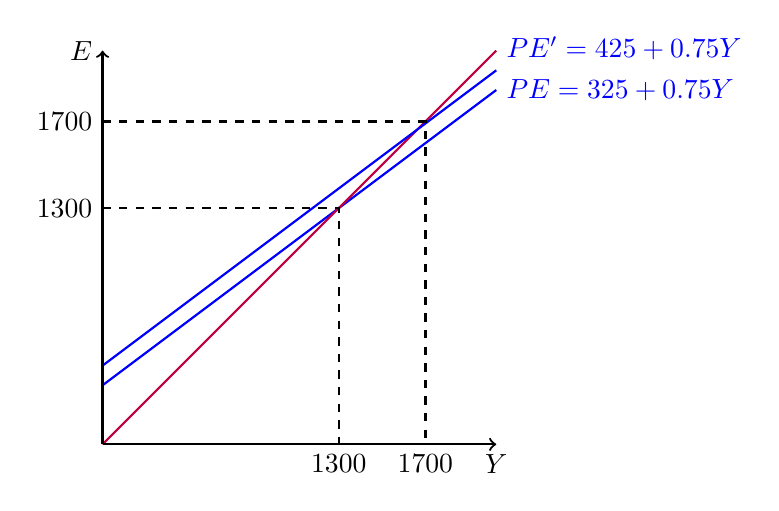
\begin{tikzpicture}[domain=0:5,scale=1,thick]
\usetikzlibrary{calc}   %allows coordinate calculations.

%Define linear parameters 
\def\dint{0.75}        %Y-intercept for DEMAND.
\def\dslp{0.75}         %Slope for DEMAND.
\def\sint{0}          %Y-intercept for SUPPLY.
\def\sslp{1}          %Slope for SUPPLY.
\def\demand{\x,{\dslp*\x+\dint}}
\def\supply{\x,{\sslp*\x+\sint}}

% Define coordinates
\coordinate (pfq) at  (3.75,0);
\coordinate (pfp) at  (3.75,3.625);
\coordinate (sfq) at  (0,3.625);

% DEMAND
\draw[thick,color=blue] plot (\demand) node[right] {$PE = 325 + 0.75Y $};

% SUPPLY
\draw[thick,color=purple] plot (\supply) ;


\draw[thick,color=blue] plot (\x,0.75*\x+1) node[above right] {$ PE' = 425 + 0.75Y $};


% Draw axes, and dotted equilibrium lines.
\draw[->] (0,0) -- (5,0) node[below] {$Y$};
\draw[->] (0,0) -- (0,5) node[left] {$E$};

%Price floor and ceiling lines
\draw[dashed] (0,3) -- (3, 3) -- (3,0) node[below] {$1300$};
\draw[dashed] (0,4.1) -- ( 4.1, 4.1) -- ( 4.1,0) node[below] {$1700$};

\node [left] at (0,4.1 ) {$ 1700 $};
\node [left] at (0,3) {$ 1300 $};

\end{tikzpicture}

The balanced
value for income: 
\begin{gather*}
E = C + I + G = 200 + 0.75 \cdot (Y - 100) + 100 + 200 = 425 + 0.75Y\\
Y = E \\
Y = 425 + 0.75Y\\
Y' = 1700
\end{gather*}
The effect of a 100 increase for public spending led to 400 increase in equilibrium output. 

\item 
The effect of a 100 increase for public spending with a same tax increase:


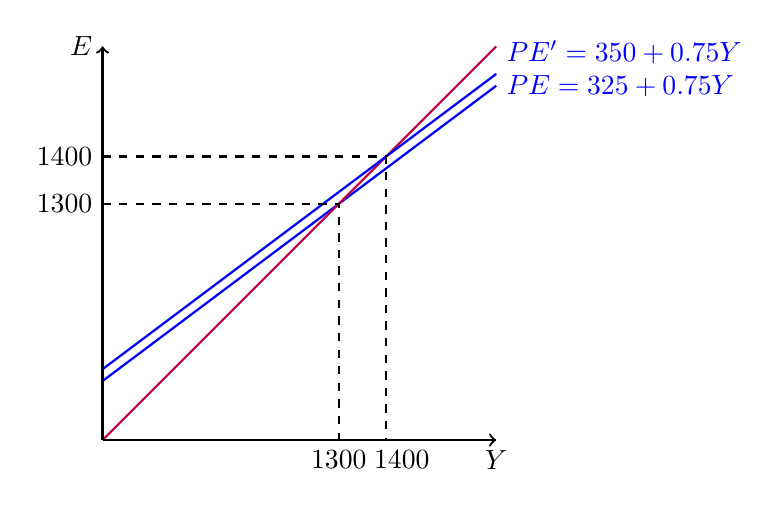
\begin{tikzpicture}[domain=0:5,scale=1,thick]
\usetikzlibrary{calc}   %allows coordinate calculations.

%Define linear parameters 
\def\dint{0.75}        %Y-intercept for DEMAND.
\def\dslp{0.75}         %Slope for DEMAND.
\def\sint{0}          %Y-intercept for SUPPLY.
\def\sslp{1}          %Slope for SUPPLY.
\def\demand{\x,{\dslp*\x+\dint}}
\def\supply{\x,{\sslp*\x+\sint}}

% Define coordinates
\coordinate (pfq) at  (3.75,0);
\coordinate (pfp) at  (3.75,3.625);
\coordinate (sfq) at  (0,3.625);

% DEMAND
\draw[thick,color=blue] plot (\demand) node[right] {$PE = 325 + 0.75Y $};

% SUPPLY
\draw[thick,color=purple] plot (\supply) ;


\draw[thick,color=blue] plot (\x,0.75*\x+0.9) node[above right] {$ PE' = 350 + 0.75Y $};


% Draw axes, and dotted equilibrium lines.
\draw[->] (0,0) -- (5,0) node[below] {$Y$};
\draw[->] (0,0) -- (0,5) node[left] {$E$};

%Price floor and ceiling lines
\draw[dashed] (0,3) -- (3, 3) -- (3,0) node[below] {$1300$};
\draw[dashed] (0,3.6) -- ( 3.6, 3.6) -- ( 3.6,0) ;

\node [left] at (0,3.6 ) {$ 1400 $};
\node [left] at (0,3) {$ 1300 $};
\node [below ]  at (3.8, 0  ) {$1400$};

\end{tikzpicture}

The balanced
value for income: 
\begin{gather*}
E = C + I + G = 200 + 0.75 \cdot (Y - 200) + 100 + 200 = 350 + 0.75Y\\
Y = E \\
Y = 350 + 0.75Y\\
Y' = 1400
\end{gather*}
The effect of a 100 increase for public spending with a same tax increase led to 100 increase in equilibrium output.


\end{enumerate}

	\item 
	The IS curve.
	
In the economy 
the macro investment function is given by the equation: $ I = 200 - 25r $ where $ r $ is the interest rate (in \%).

 \begin{enumerate} [label=\arabic*)] 
	\setcounter{enumii}{7}

\item In the Keynesian cross model, an increase in interest rate leads to a decrease in investment, which leads to a decrease in equilibrium level of output.  

\item Investment functions, one where investment is not affected by changes in
interest rate and one where it is:


\begin{tikzpicture}[domain=0:5,scale=1,thick]
\usetikzlibrary{calc}   %allows coordinate calculations.


\draw[thick,color=purple] (6,4) -- (10,1) node [right] {$I(r)$} ;
\draw[thick,color=purple] (0,2.5) -- (4.5,2.5) node [right] {$I(r)$} ;

% Draw axes, and dotted equilibrium lines.
\draw[->] (0,0) -- (5,0) node[below] {$r$};
\draw[->] (0,0) -- (0,5) node[left] {$I$};

% Draw axes, and dotted equilibrium lines.
\draw[->] (6,0) -- (6,5) node[left] {$I$};
\draw[->] (6,0) -- (11,0) node[below] {$r$};



\end{tikzpicture}

In case,  where investment is not affected by changes in
interest rate (shown in the left graph), changes in interest rate do not influence the amount of investments and thus do not influence equilibrium level of output.   And where investment is affected by changes in
interest rate (shown in the right graph),  the consequences of higher interest rate are increased level of investments and thus increased level of output. 
That can be shown using the $ 45\degree $  diagram.


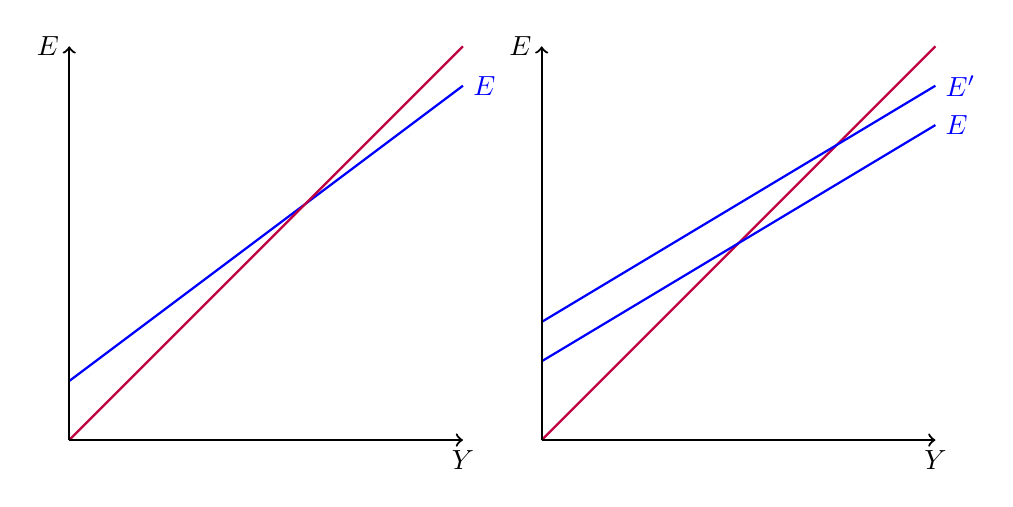
\begin{tikzpicture}[domain=0:5,scale=1,thick]
\usetikzlibrary{calc}   %allows coordinate calculations.

%Define linear parameters 
\def\dint{0.75}        %Y-intercept for DEMAND.
\def\dslp{0.75}         %Slope for DEMAND.
\def\sint{0}          %Y-intercept for SUPPLY.
\def\sslp{1}          %Slope for SUPPLY.
\def\demand{\x,{\dslp*\x+\dint}}
\def\supply{\x,{\sslp*\x+\sint}}

% Define coordinates
\coordinate (pfq) at  (3.75,0);
\coordinate (pfp) at  (3.75,3.625);
\coordinate (sfq) at  (0,3.625);

\draw[thick,color=blue] plot (\demand) node[right] {$E$};
\draw[thick,color=purple] plot (\supply);

\draw[thick,color=purple] (6,0) -- (11,5) ;
\draw[thick,color=blue] (6,1) -- (11,4) node[right] {$E$};
\draw[thick,color=blue] (6,1.5) -- (11,4.5) node[right] {$E'$};


% Draw axes, and dotted equilibrium lines.
\draw[->] (0,0) -- (5,0) node[below] {$Y$};
\draw[->] (0,0) -- (0,5) node[left] {$E$};

% Draw axes, and dotted equilibrium lines.
\draw[->] (6,0) -- (6,5) node[left] {$E$};
\draw[->] (6,0) -- (11,0) node[below] {$Y$};

\end{tikzpicture}

\newpage

\item  The equation of the IS curve for this economy:
\begin{gather}
E = C + I + G = 200 + 0.75 \cdot (Y - 100) + 200 - 25r + 100 = 425 + 0.75Y - 25r\\
Y = E \\
Y =  425 + 0.75Y - 25r \\
r = 17 - 0.01Y
\end{gather} 
\item A  graph for the IS curve: 

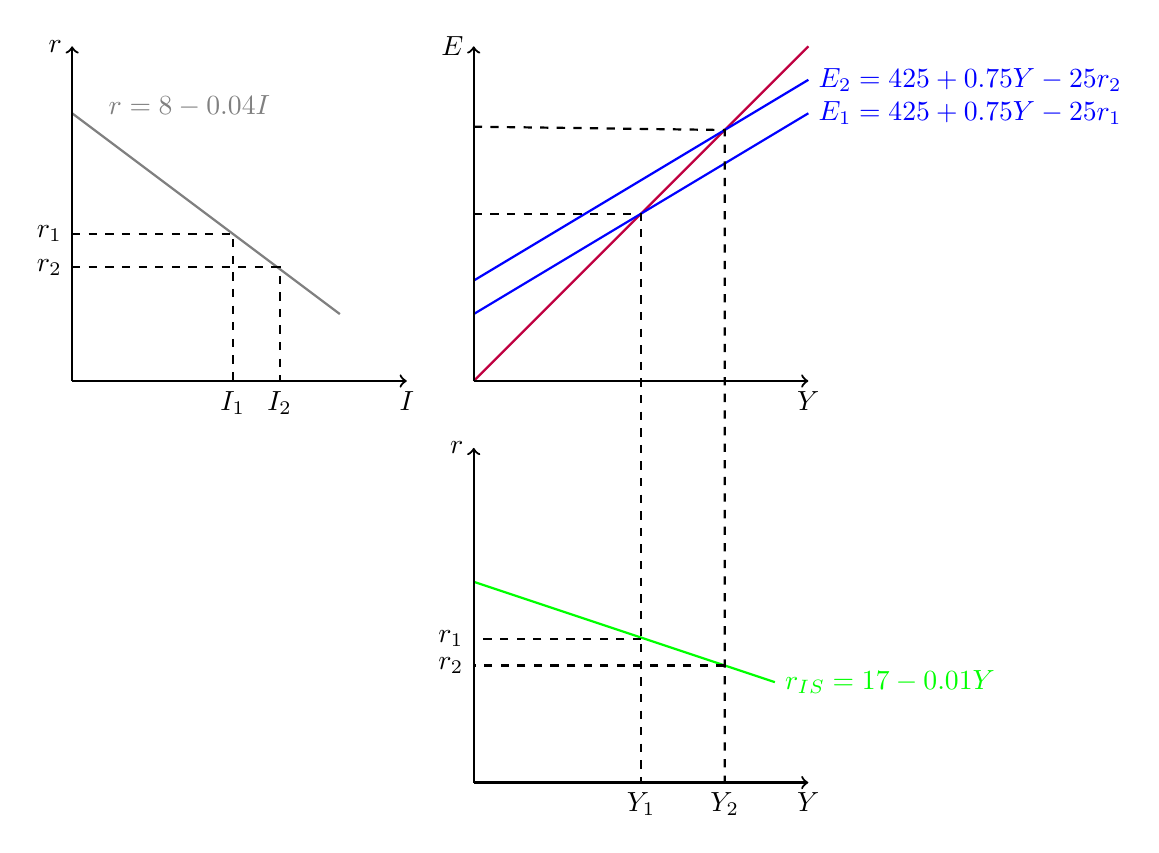
\begin{tikzpicture}[domain=0:5,scale=0.85,thick]
\usetikzlibrary{calc}   %allows coordinate calculations.

\draw[thick,color=gray] (0,4) -- (4,1)  ;
\draw[thick,color=purple] (6,0) -- (11,5) ;
\draw[thick,color=blue] (6,1) -- (11,4) node[right] {$E_{1} = 425 + 0.75Y - 25r_{1} $};
\draw[thick,color=blue] (6,1.5) -- (11,4.5) node[right] {$E_{2} = 425 + 0.75Y - 25r_{2} $};
\draw[thick,color=green] (6,-3) -- (10.5,-4.5) node[right] {$r_{IS} = 17 - 0.01Y $} ;


% Draw axes, and dotted equilibrium lines.
\draw[->] (0,0) -- (5,0) node[below] {$I$};
\draw[->] (0,0) -- (0,5) node[left] {$r$};

% Draw axes, and dotted equilibrium lines.
\draw[->] (6,0) -- (6,5) node[left] {$E$};
\draw[->] (6,0) -- (11,0) node[below] {$Y$};

% Draw axes, and dotted equilibrium lines.
\draw[->] (6,-6) -- (6,-1) node[left] {$r$};
\draw[->] (6,-6) -- (11,-6) node[below] {$Y$};

\draw[dashed] (0,2.2) -- (2.4, 2.2) -- (2.4,0) node[below] {$I_{1}$};
\draw[dashed] (0,1.7) -- ( 3.1, 1.7) -- ( 3.1,0) node[below] {$I_{2}$};

\draw[dashed] (6,2.5) -- (8.5, 2.5) -- (8.5,-6) node[below] {$Y_{1}$};
\draw[dashed] (6,3.8) -- (9.75, 3.75) -- ( 9.75,-6) node[below] {$Y_{2}$};

\draw[dashed] (8.5, -3.85) -- (6,-3.85) node[left] {$r_{1}$};
\draw[dashed] ( 9.75,-4.25) -- (6, -4.25)   node[left] {$r_{2}$};

\node [color=gray] at (1.75,4.1) {$r = 8 - 0.04I $};
\node [left] at (0,2.2 ) {$ r_{1} $};
\node [left] at (0,1.7) {$ r_{2} $};
\end{tikzpicture}
\item  The effect of a 50 cut in public spending.

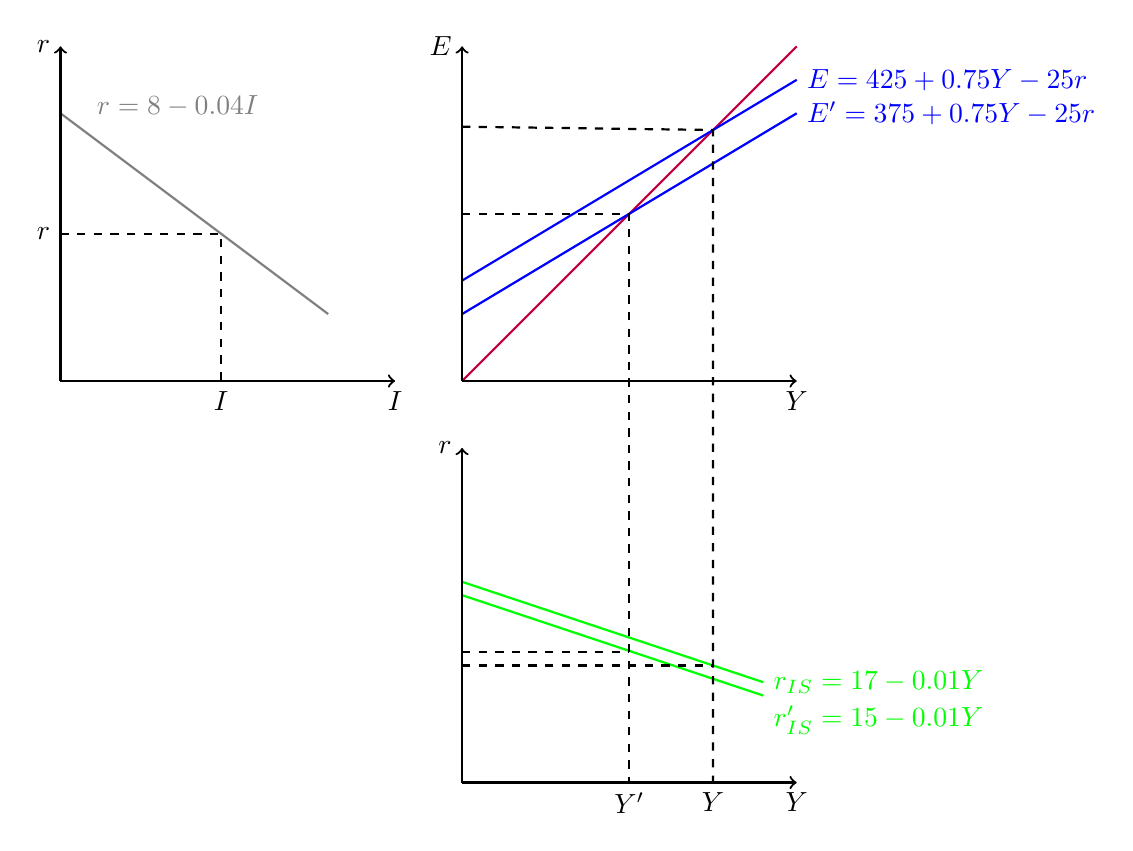
\begin{tikzpicture}[domain=0:5,scale=0.85,thick]
\usetikzlibrary{calc}   %allows coordinate calculations.

\draw[thick,color=gray] (0,4) -- (4,1)  ;
\draw[thick,color=purple] (6,0) -- (11,5) ;
\draw[thick,color=blue] (6,1) -- (11,4) node[right] {$E' = 375 + 0.75Y - 25r $};
\draw[thick,color=blue] (6,1.5) -- (11,4.5) node[right] {$E = 425 + 0.75Y - 25r $};
\draw[thick,color=green] (6,-3) -- (10.5,-4.5) node[right] {$r_{IS} = 17 - 0.01Y $} ;
\draw[thick,color=green] (6,-3.2) -- (10.5,-4.7) node[below right] {$r'_{IS} = 15 - 0.01Y $} ;


% Draw axes, and dotted equilibrium lines.
\draw[->] (0,0) -- (5,0) node[below] {$I$};
\draw[->] (0,0) -- (0,5) node[left] {$r$};

% Draw axes, and dotted equilibrium lines.
\draw[->] (6,0) -- (6,5) node[left] {$E$};
\draw[->] (6,0) -- (11,0) node[below] {$Y$};

% Draw axes, and dotted equilibrium lines.
\draw[->] (6,-6) -- (6,-1) node[left] {$r$};
\draw[->] (6,-6) -- (11,-6) node[below] {$Y$};

\draw[dashed] (0,2.2) -- (2.4, 2.2) -- (2.4,0) node[below] {$I$};

\draw[dashed] (6,2.5) -- (8.5, 2.5) -- (8.5,-6) node[below] {$Y'$};
\draw[dashed] (6,3.8) -- (9.75, 3.75) -- ( 9.75,-6) node[below] {$Y$};
\draw[dashed] (6,-4.25) -- (9.75, -4.25) ;
\draw[dashed] (6,-4.05) -- (8.5, -4.05) ;


%\draw[dashed] (8.5, -3.85) -- (6,-3.85) ;
%\draw[dashed] ( 9.75,-4.45) -- (6, -4.45)  ;

\node [color=gray] at (1.75,4.1) {$r = 8 - 0.04I $};

\node [left] at (0,2.2 ) {$ r $};


\end{tikzpicture}



\item  The effect of 50 increase in the available quantity of money:


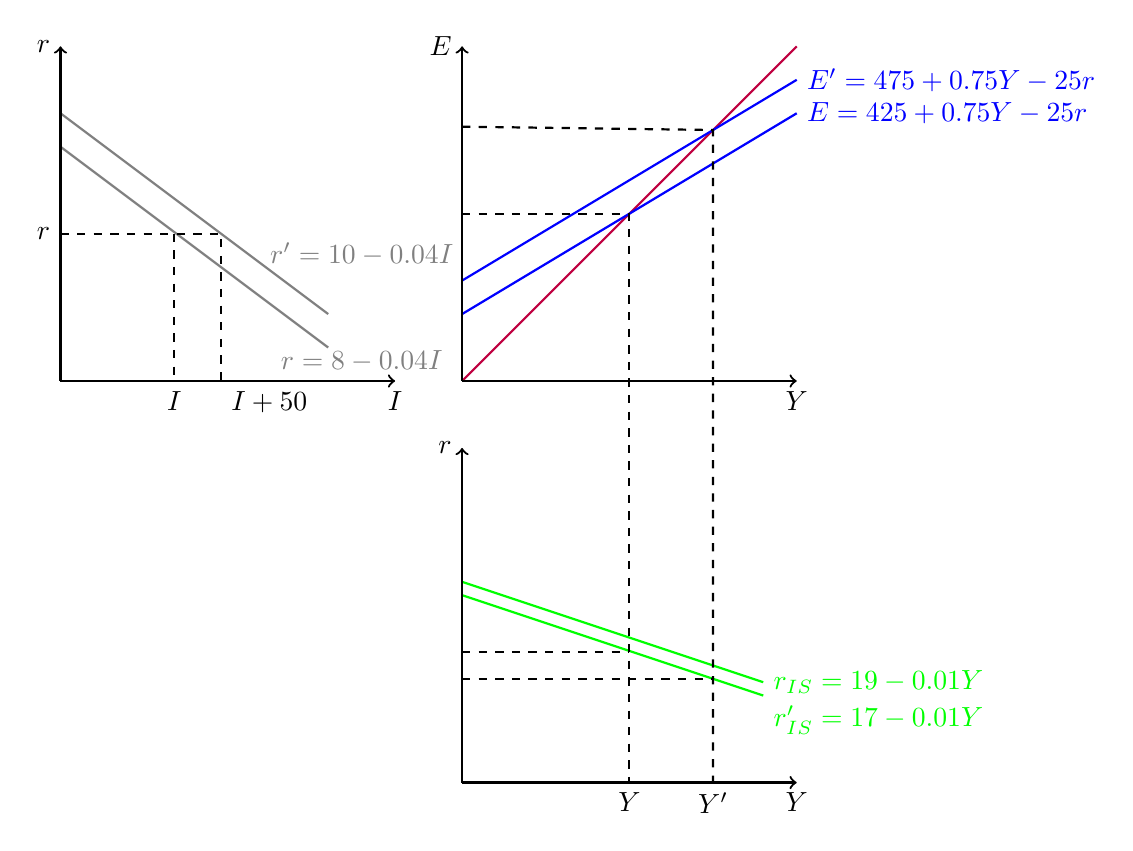
\begin{tikzpicture}[domain=0:5,scale=0.85,thick]
\usetikzlibrary{calc}   %allows coordinate calculations.

\draw[thick,color=gray] (0,4) -- (4,1)  ;
\draw[thick,color=gray] (0,3.5) -- (4,0.5)  ;

\draw[thick,color=purple] (6,0) -- (11,5) ;
\draw[thick,color=blue] (6,1) -- (11,4) node[right] {$E = 425 + 0.75Y - 25r $};
\draw[thick,color=blue] (6,1.5) -- (11,4.5) node[right] {$E' = 475 + 0.75Y - 25r $};
\draw[thick,color=green] (6,-3) -- (10.5,-4.5) node[right] {$r_{IS} = 19 - 0.01Y $} ;
\draw[thick,color=green] (6,-3.2) -- (10.5,-4.7) node[below right] {$r'_{IS} = 17 - 0.01Y $} ;


% Draw axes, and dotted equilibrium lines.
\draw[->] (0,0) -- (5,0) node[below] {$I$};
\draw[->] (0,0) -- (0,5) node[left] {$r$};

% Draw axes, and dotted equilibrium lines.
\draw[->] (6,0) -- (6,5) node[left] {$E$};
\draw[->] (6,0) -- (11,0) node[below] {$Y$};

% Draw axes, and dotted equilibrium lines.
\draw[->] (6,-6) -- (6,-1) node[left] {$r$};
\draw[->] (6,-6) -- (11,-6) node[below] {$Y$};

\draw[dashed] (0,2.2) -- (2.4, 2.2) -- (2.4,0) node[below right] {$I+50$};
\draw[dashed]  (1.7, 2.2) -- (1.7,0) node[below] {$I$};

\draw[dashed] (6,2.5) -- (8.5, 2.5) -- (8.5,-6) node[below] {$Y$};
\draw[dashed] (6,3.8) -- (9.75, 3.75) -- ( 9.75,-6) node[below] {$Y'$};
\draw[dashed] (6,-4.45) -- (9.75, -4.45) ;
\draw[dashed] (6,-4.05) -- (8.5, -4.05) ;


%\draw[dashed] (8.5, -3.85) -- (6,-3.85) node[left] {$r$};
%\draw[dashed] ( 9.75,-4.45) -- (6, -4.45)   node[left] {$r'$};

\node [color=gray] at (4.5,0.3) {$r = 8 - 0.04I $};
\node [color=gray] at (4.5,1.9) {$r' = 10 - 0.04I $};

\node [left] at (0,2.2 ) {$ r $};


\end{tikzpicture}



\end{enumerate}


	\item 
 The LM curve.
	

In the economy  
the function of money demand is $ \dfrac{M^{d}}{P} = Y - 100r $ with r the interest rate (in \%), nominal money supply $ M = 1000  $ and the
price level is $  P = 2 $.


\begin{enumerate} [label=\arabic*)] 
	\setcounter{enumii}{13}


\item  The money supply is  $ \dfrac{M^{s}}{P} =  \dfrac{1000}{2} = 500 $, and since $ \frac{M^{d}}{P} = \frac{M^{s}}{P}  $ the value of real money balances available in the economy equals 500.

\item  Equilibrium on the money
market will be:
\begin{gather}
\dfrac{M^{d}}{P} = \dfrac{M^{s}}{P} \\  
Y - 100r = 500 
\end{gather}
If global income is equal to 1000, the equilibrium interest rate: 
\begin{gather}
Y_{1}=1000 \\  
1000 - 100r = 500 \\
r_{1}=5
\end{gather}
If global income is equal to 2000, the equilibrium interest rate: 
\begin{gather}
Y_{1}=2000 \\  
2000 - 100r = 500 \\
r_{2}=15
\end{gather}
\newpage
\item  The money market diagram:

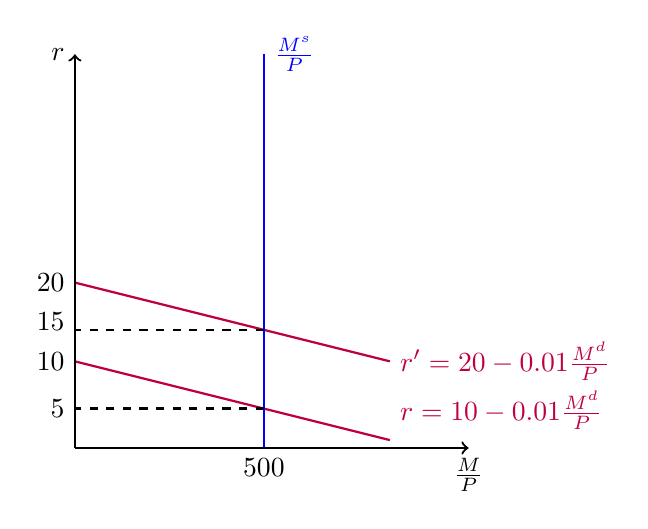
\begin{tikzpicture}[domain=0:5,scale=1,thick]
\usetikzlibrary{calc}   %allows coordinate calculations.

\draw[thick,color=purple] (0,3.5) -- (4,2.5) node[right] {$r'=20-0.01\frac{M^{d}}{P}$ };
\draw[thick,color=purple] (0,2.5) -- (4,1.5) node[above right] {$r=10-0.01\frac{M^{d}}{P}$ };
\draw[thick,color=blue]  (2.4,1.4)--(2.4, 6.4) node[ right] {$\frac{M^{s}}{P}$};

% Draw axes, and dotted equilibrium lines.
\draw[->] (0,1.4) -- (5,1.4) node[below] {$\frac{M}{P}$};
\draw[->] (0,1.4) -- (0,6.4) node[left] {$r$};

\draw[dashed] (2.4, 2.9) -- (0,2.9)  ;
\draw[dashed]  (2.4, 1.9) -- (0,1.9) ;
\node [left] at (0,3.5 ) {$ 20 $};
\node [left] at (0,2.5 ) {$ 10 $};
\node [left] at (0,3 ) {$ 15 $};
\node [left] at (0,1.9 ) {$ 5 $};
\node [below] at (2.4,1.4) {$ 500 $};
\end{tikzpicture}


\item LM curve for this economy:
\begin{gather}
\dfrac{M^{d}}{P} = \dfrac{M^{s}}{P} \\  
Y - 100r = 500\\
r=0.01Y-5 
\end{gather}
\item  A  graph for the LM curve: 

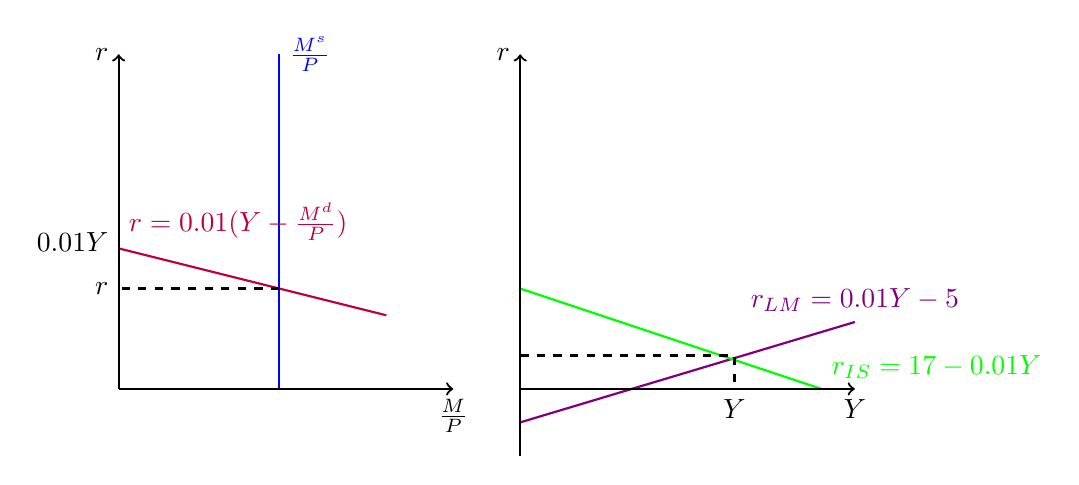
\begin{tikzpicture}[domain=0:5,scale=0.85,thick]
\usetikzlibrary{calc}   %allows coordinate calculations.

\draw[thick,color=purple] (0,2.1) -- (4,1.1) ;
\draw[thick,color=blue]  (2.4,0)--(2.4, 5) node[ right] {$\frac{M^{s}}{P}$};

% Draw axes, and dotted equilibrium lines.
\draw[->] (0,0) -- (5,0) node[below] {$\frac{M}{P}$};
\draw[->] (0,0) -- (0,5) node[left] {$r$};

\draw[thick,color=violet] (6,-0.5) -- (11,1) node[above] {$r_{LM} = 0.01Y - 5  $};
\draw[thick,color=green] (6,1.5) -- (10.5,0) node[above right] {$r_{IS} = 17 - 0.01Y $} ;

% Draw axes, and dotted equilibrium lines.
\draw[->] (6,-1) -- (6,5) node[left] {$r$};
\draw[->] (6,0) -- (11,0) node[below] {$Y$};

\draw[dashed] (2.4, 1.5 ) -- (0,1.5 )  node[left] {$r$};

\draw[dashed] (6,0.5) -- (9.2, 0.5) -- ( 9.2,0) node[below] {$Y$};

\node [right, color=purple] at (0,2.5) {$r=0.01(Y-\frac{M^{d}}{P})$ };
\node [left] at (0,2.2 ) {$ 0.01Y $};
%\node [left] at (6,0.5) {$ r $};
\end{tikzpicture}

\item The effect of an increase in the quantity of money on the money market is a shift of money supply curve to the right, 
LM curve will also be shifted to the right (with lower equilibrium interest rate and higher output):

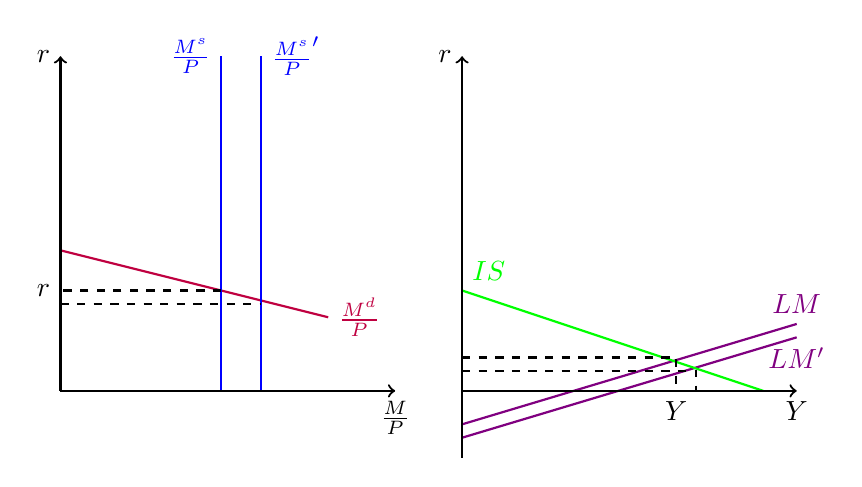
\begin{tikzpicture}[domain=0:5,scale=0.85,thick]
\usetikzlibrary{calc}   %allows coordinate calculations.

\draw[thick,color=purple] (0,2.1) -- (4,1.1) node [right] {$\frac{M^{d}}{P}$} ;
\draw[thick,color=blue]  (2.4,0)--(2.4, 5) node[ left] {$\frac{M^{s}}{P}$};
\draw[thick,color=blue]  (3,0)--(3, 5) node[ right] {$\frac{M^{s}}{P}'$};


% Draw axes, and dotted equilibrium lines.
\draw[->] (0,0) -- (5,0) node[below] {$\frac{M}{P}$};
\draw[->] (0,0) -- (0,5) node[left] {$r$};

\draw[thick,color=violet] (6,-0.5) -- (11,1) node[above] {$LM $};
\draw[thick,color=violet] (6,-0.7) -- (11,0.8) node[below] {$LM' $};

\draw[thick,color=green] (10.5,0)--(6,1.5)  node[above right] {$IS $} ;

% Draw axes, and dotted equilibrium lines.
\draw[->] (6,-1) -- (6,5) node[left] {$r$};
\draw[->] (6,0) -- (11,0) node[below] {$Y$};

\draw[dashed] (2.4, 1.5 ) -- (0,1.5 )  node[left] {$r$};
\draw[dashed] (0,1.3 ) -- (3, 1.3 )  ;


\draw[dashed] (6,0.5) -- (9.2, 0.5) -- ( 9.2,0) node[below] {$Y$};

\draw[dashed] (6,0.3) -- (9.5, 0.3) -- ( 9.5,0) ;


%\node [left] at (0,2.2 ) {$ 0.01Y $};
%\node [left] at (6,0.5) {$ r_{2} $};
\end{tikzpicture}



\item  An increase in government spending will not affect LM curve, but IS curve will shift to the right (which will lead to higher equilibrium interest rate and output)


\end{enumerate}

\item IS-LM and the aggregate demand. 

The economy we have can be described by the following equations: the consumption function $ C = 200 + 0.75(Y - T) $, the government budget is balanced, so $ G=T=100 $, the investment function $ I = 200 - 25r $, the real money
demand 
$ \frac{M^{d}}{P} = Y - 100r $, the real money supply $ \frac{M^{s}}{P} = \frac{1000}{2} = 500  $.

\begin{enumerate} [label=\arabic*)] 
	\setcounter{enumii}{20}

\item   IS-LM  diagram: 

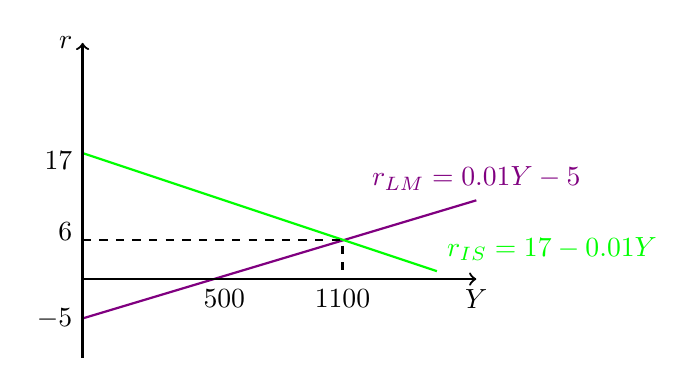
\begin{tikzpicture}[domain=0:5,scale=1,thick]
\usetikzlibrary{calc}   %allows coordinate calculations.


\draw[thick,color=violet] (6,-0.5) -- (11,1) node[above] {$r_{LM} = 0.01Y - 5  $};
\draw[thick,color=green] (6,1.6) -- (10.5,0.1) node[above right] {$r_{IS} = 17 - 0.01Y $} ;

% Draw axes, and dotted equilibrium lines.
\draw[->] (6,-1) -- (6,3) node[left] {$r$};
\draw[->] (6,0) -- (11,0) node[below] {$Y$};

%\draw[dashed] (2.4, 1.5 ) -- (0,1.5 )  node[left] {$r$};

\draw[dashed] (6,0.5) -- (9.3, 0.5) -- ( 9.3,0) node[below] {$1100$};

\node [left] at (6,1.5 ) {$ 17 $};
\node [left] at (6,0.6) {$ 6 $};
\node [left] at (6,-0.5) {$ -5 $};
\node [below] at (7.8,0 ) {$ 500 $};


\end{tikzpicture}



\item   IS-LM system of equations give the following values of income $ Y $ and interest rate $ r $  in a
situation of balanced markets for goods and services and for money (for IS equation derivation see 10, for LM - see 17). 
\begin{gather}
IS: r = 17 - 0.01Y \\
LM: r =  0.01Y - 5 \\
17 - 0.01Y = 0.01Y - 5 \\
Y = 1100 \Rightarrow r = 6 \\
\end{gather} 
This result is also graphically
represented (see 21).

\item  The government spending increases from 100 to 150, as a result both the new income
and interest rate values rise:
\begin{gather}
IS: Y=E \Rightarrow Y = C + I + G \Rightarrow Y = 200 + 0.75 \cdot (Y - 100) + 200 - 25r + 150 \\
Y =  475 + 0.75Y - 25r\\
r = 19 - 0.01Y \\
LM: r =  0.01Y - 5 \\
19 - 0.01Y = 0.01Y - 5 \\
Y = 1200 \Rightarrow r = 7 \\
\end{gather} 
\item  The value of the, for instance, government spending multiplier is: 
\begin{gather}
IS: Y = C + I + G \Rightarrow Y = C_{0} + MPC \cdot (Y - T) + I_{0} - b \cdot r + G \\
LM: \frac{M^{d}}{P} = \frac{M^{s}}{P} \Rightarrow Y - c \cdot r = \frac{M^{s}}{P}  \Rightarrow Y =  \frac{M^{s}}{P} + c \cdot r \\
\dfrac{-Y + C_{0} + MPC \cdot Y - MPC \cdot T + I_{0}  + G}{b} = \dfrac{Y - \frac{M^{s}}{P} }{c} \\
Y = \dfrac{b(C_{0}  - MPC \cdot T + I_{0}  + G) + c\frac{M^{s}}{P} }{ c  + b - MPC} \\
\dfrac{\partial Y}{\partial G} =  \dfrac{b \cdot G }{ c  + b - MPC} 
\end{gather} 
This value is different from the one obtained with the
Keynesian cross model, since investment function depend on interest rate and balanced value of output depend on equilibrium on money market. The parameters which make the results different are $ b $ - sensitivity coefficient of  investment level to interest rate and $ c $ -  sensitivity coefficient of  money demand to interest rate.

\item  The government is maintaining its budget policy and the central bank decides to increase the
money supply from 1000 to 1200. The new situation for the economy:  
\begin{gather}
IS: r = 17 - 0.01Y\\
LM: \frac{M^{d}}{P} = \frac{M^{s}}{P} \Rightarrow Y - 100r = \frac{1000}{2} \Rightarrow r =  0.01Y - 6 \\
17 - 0.01Y = 0.01Y - 6 \\
Y = 1150 \Rightarrow r = 5.5 \\
\end{gather} 
\item  An inflationary shock increases the price index from 2 to 4. The new situation for the
economy: 
\begin{gather}
IS: r = 17 - 0.01Y\\
LM: \frac{M^{d}}{P} = \frac{M^{s}}{P} \Rightarrow Y - 100r = \frac{1000}{4} \Rightarrow r =  0.01Y - 2.5 \\
17 - 0.01Y = 0.01Y - 2.5 \\
Y = 975 \Rightarrow r = 7.25 \\
\end{gather} 



\end{enumerate}


\end{enumerate}

\end{document}